\subsection{Iteration \#1}
I iteration 1 arbejdes der med blokke som dækker over systemets mest grundlæggende funktionalitet. Batteri, ESC’er, motorer og sensorer tilsluttes dronen, og dronen gøres desuden i stand til oprette forbindelse til webapplikationen via 3G-shield’et.
Server opsættes, så at basal kommunikation mellem dronen og server er muligt. Det skal bla. være muligt for dronen at uploade sin nuværende position til server. For flere detaljer vedrørende opsætning og funktionalitet af server henvises til data view'et. 
Hvordan systemet er tiltænkt at bruges beskrives i user story nedenfor:

\subsubsection*{User story}
Bruger tænder dronen ved at tilslutte batteri. Main controller samt 3G/GPS module initialiseres og nuværende GPS position opdateres. Herefter oprettes forbindelse mellem drone og websitet, og information om dronen er online samt information om dronens nuværende GPS position sendes til websitet. Fra websitet er det muligt for bruger løbende at observere hvorvidt dronen er online og på hvilken GPS position dronen sidst har befundet sig.

%kommentar
\begin{figure}[H]
	\centering
	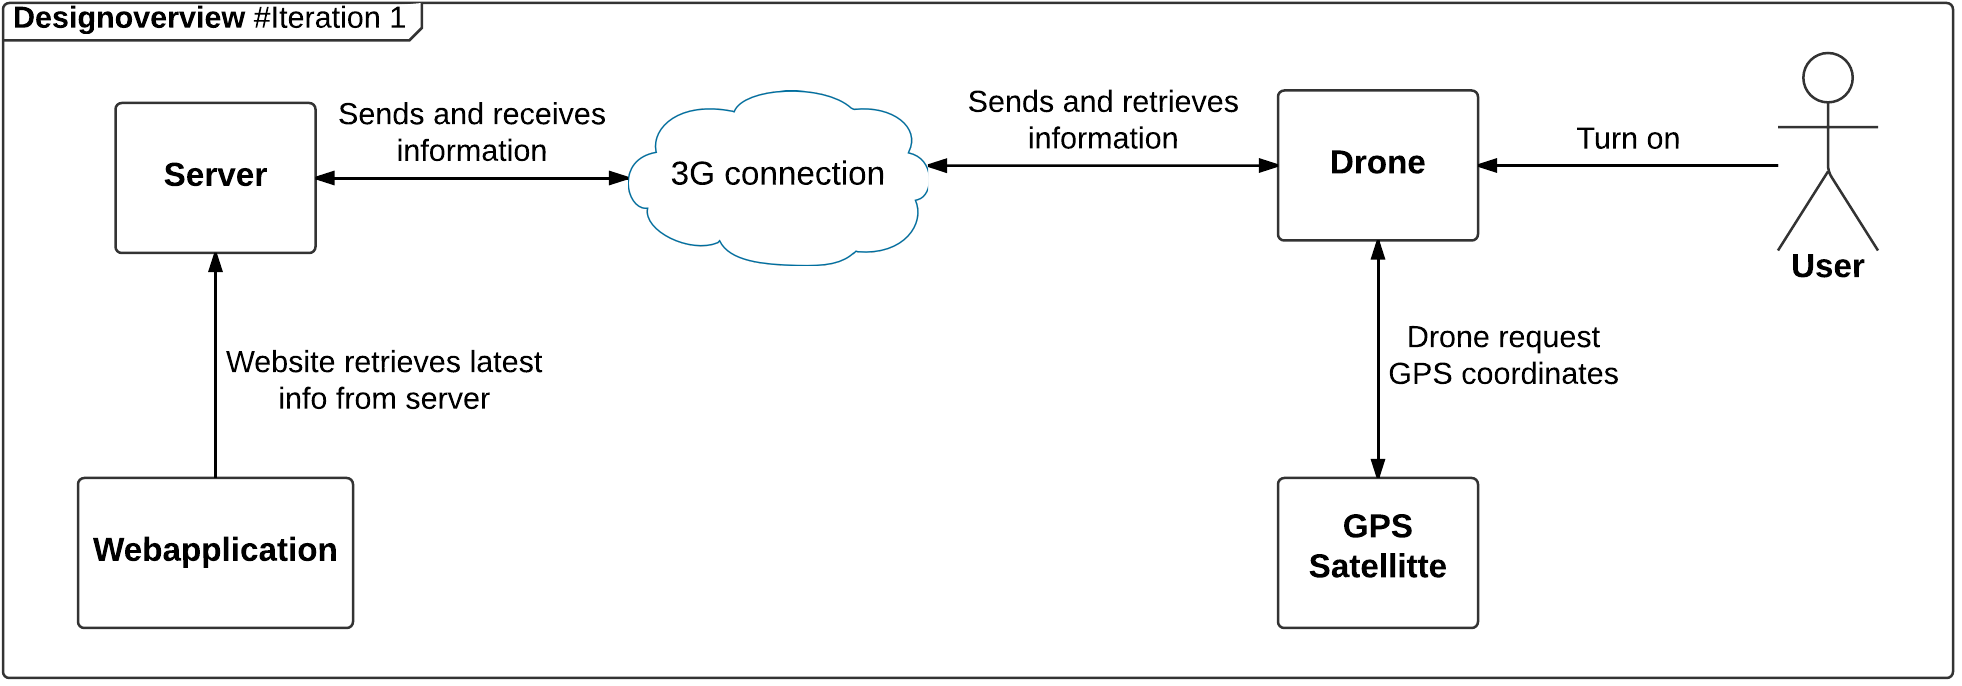
\includegraphics[width=1\textwidth]{Billeder/design_overview/design_overview_iteration1.png}
	\vspace{-.5cm}
	\caption{Design overview \#iteration 1}
	\label{fig:design_overview_UC1}
\end{figure}


\newpage
\subsubsection*{Pakke diagram Drone}

I denne sektion vises pakkediagrammer tilhørende drone. De pakker der vises i pakkediagrammerne består af en eller flere klasser, der med stort samspil udfører opgaver indenfor et fælles ansvarsområde. På hver pakke findes en lille beskrivelse, der tydeliggør pakkens ansvarsområde. 


\begin{figure}[H]
	\centering
	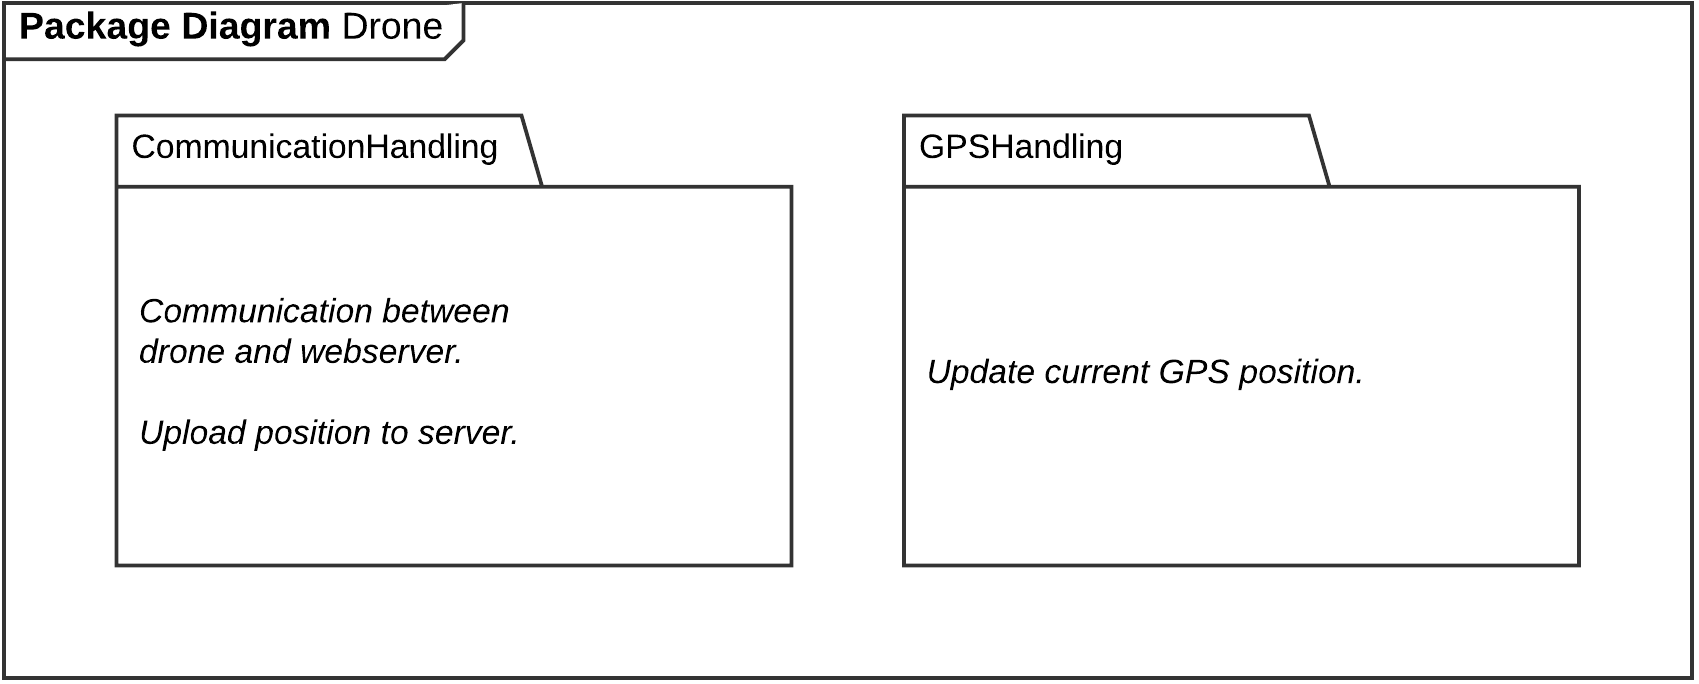
\includegraphics[width=1\textwidth]{Billeder/pakke_diagrammer/iteration1_drone.png}
	\vspace{-0.5cm}
	\caption{Pakkediagram drone}
	\label{fig:iteration1_pakke_diagram_drone}
\end{figure}

\textbf{CommunicationHandling}\\
Pakkens ansvar er kommunikation imellem drone og server. Der er fokus på at drone kan sende GPS position til server.

\textbf{SensorHandling}\\
Pakkens ansvar er håndtering af 3G, GPS og højdesensor data.


\newpage
\subsubsection*{Pakke diagram Webapplikation}

I denne sektion vises pakkediagrammer tilhørende drone. De pakker der vises i pakkediagrammerne består af en eller flere klasser, der med stort samspil udfører opgaver indenfor et fælles ansvarsområde. På hver pakke findes en lille beskrivelse, der tydeliggør pakkens ansvarsområde.

\begin{figure}[H]
	\centering
	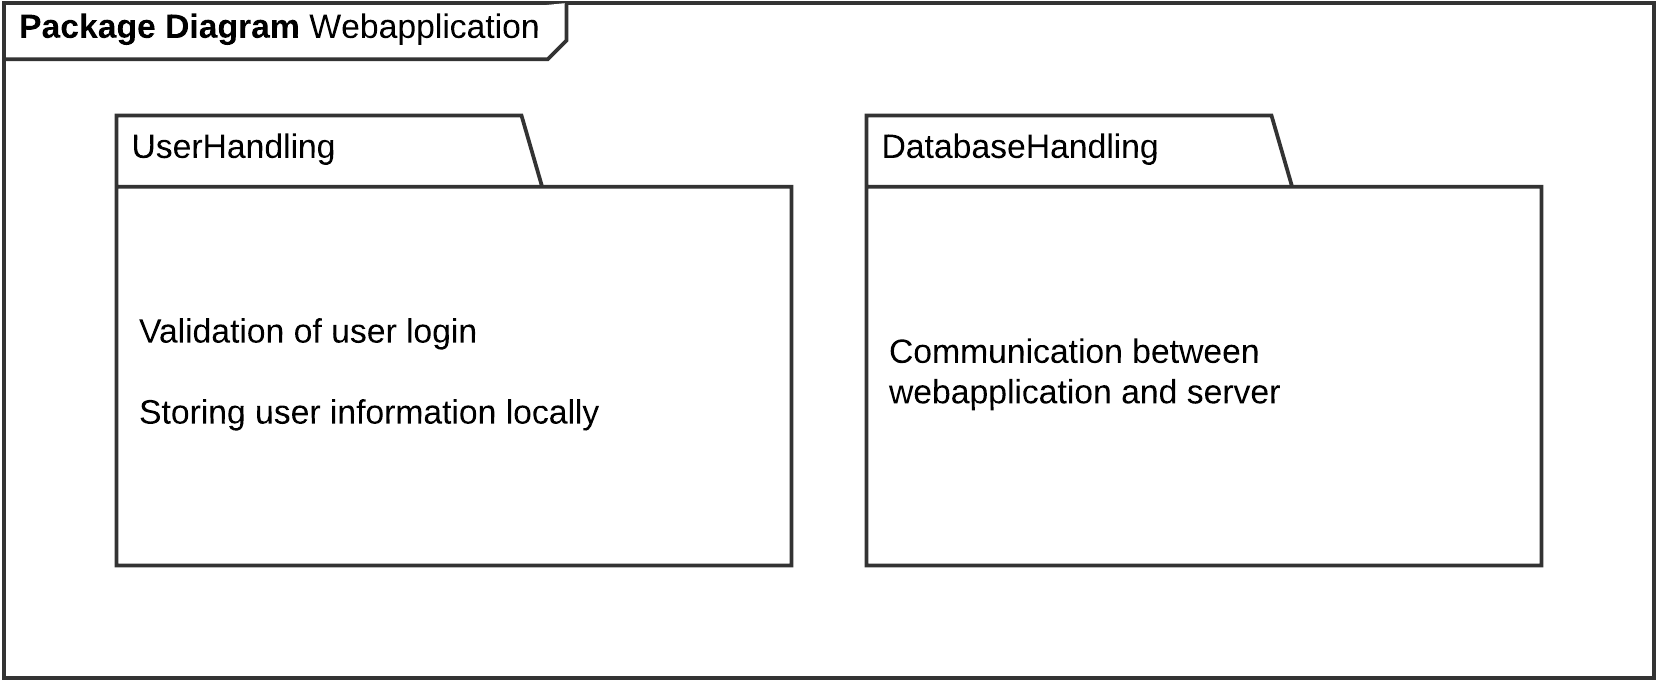
\includegraphics[width=1\textwidth]{Billeder/pakke_diagrammer/iteration1_server.png}
	\vspace{-0.5cm}
	\caption{Overordnet pakke diagram over webapplikationen}
	\label{fig:iteration1_pakke_diagram_webapp}
\end{figure}

\textbf{CommunicationHandling}\\
Pakkens ansvar er kommunikation imellem drone og server. Pakken sender flyveinformation til dronen, som bruger har lavet på webapplikationen.

\textbf{UserHandling}\\
Pakkens ansvar er validering af login/log ud på websitet. Pakken har også ansvaret for at hente og gemme data om den pågældende bruger.

\textbf{DatabaseHandling}\\
Pakkens ansvar er kommunikation imellem databasen og serveren. 


\newpage

\subsubsection*{Klasse diagram - drone}
\vspace{-0.2cm}
Figur \ref{fig:classDiagram_iteration1} vises et klassediagram tilhørende iteration 1. Klassediagrammet viser iterationens vigtigste klasser, samt deres tilhørende metoder og attributter. På den følgende side forefindes en kort beskrivelse klasserne og deres metoder.

\vspace{-0.2cm}
%kommentar
\begin{figure}[H]
	\centering
	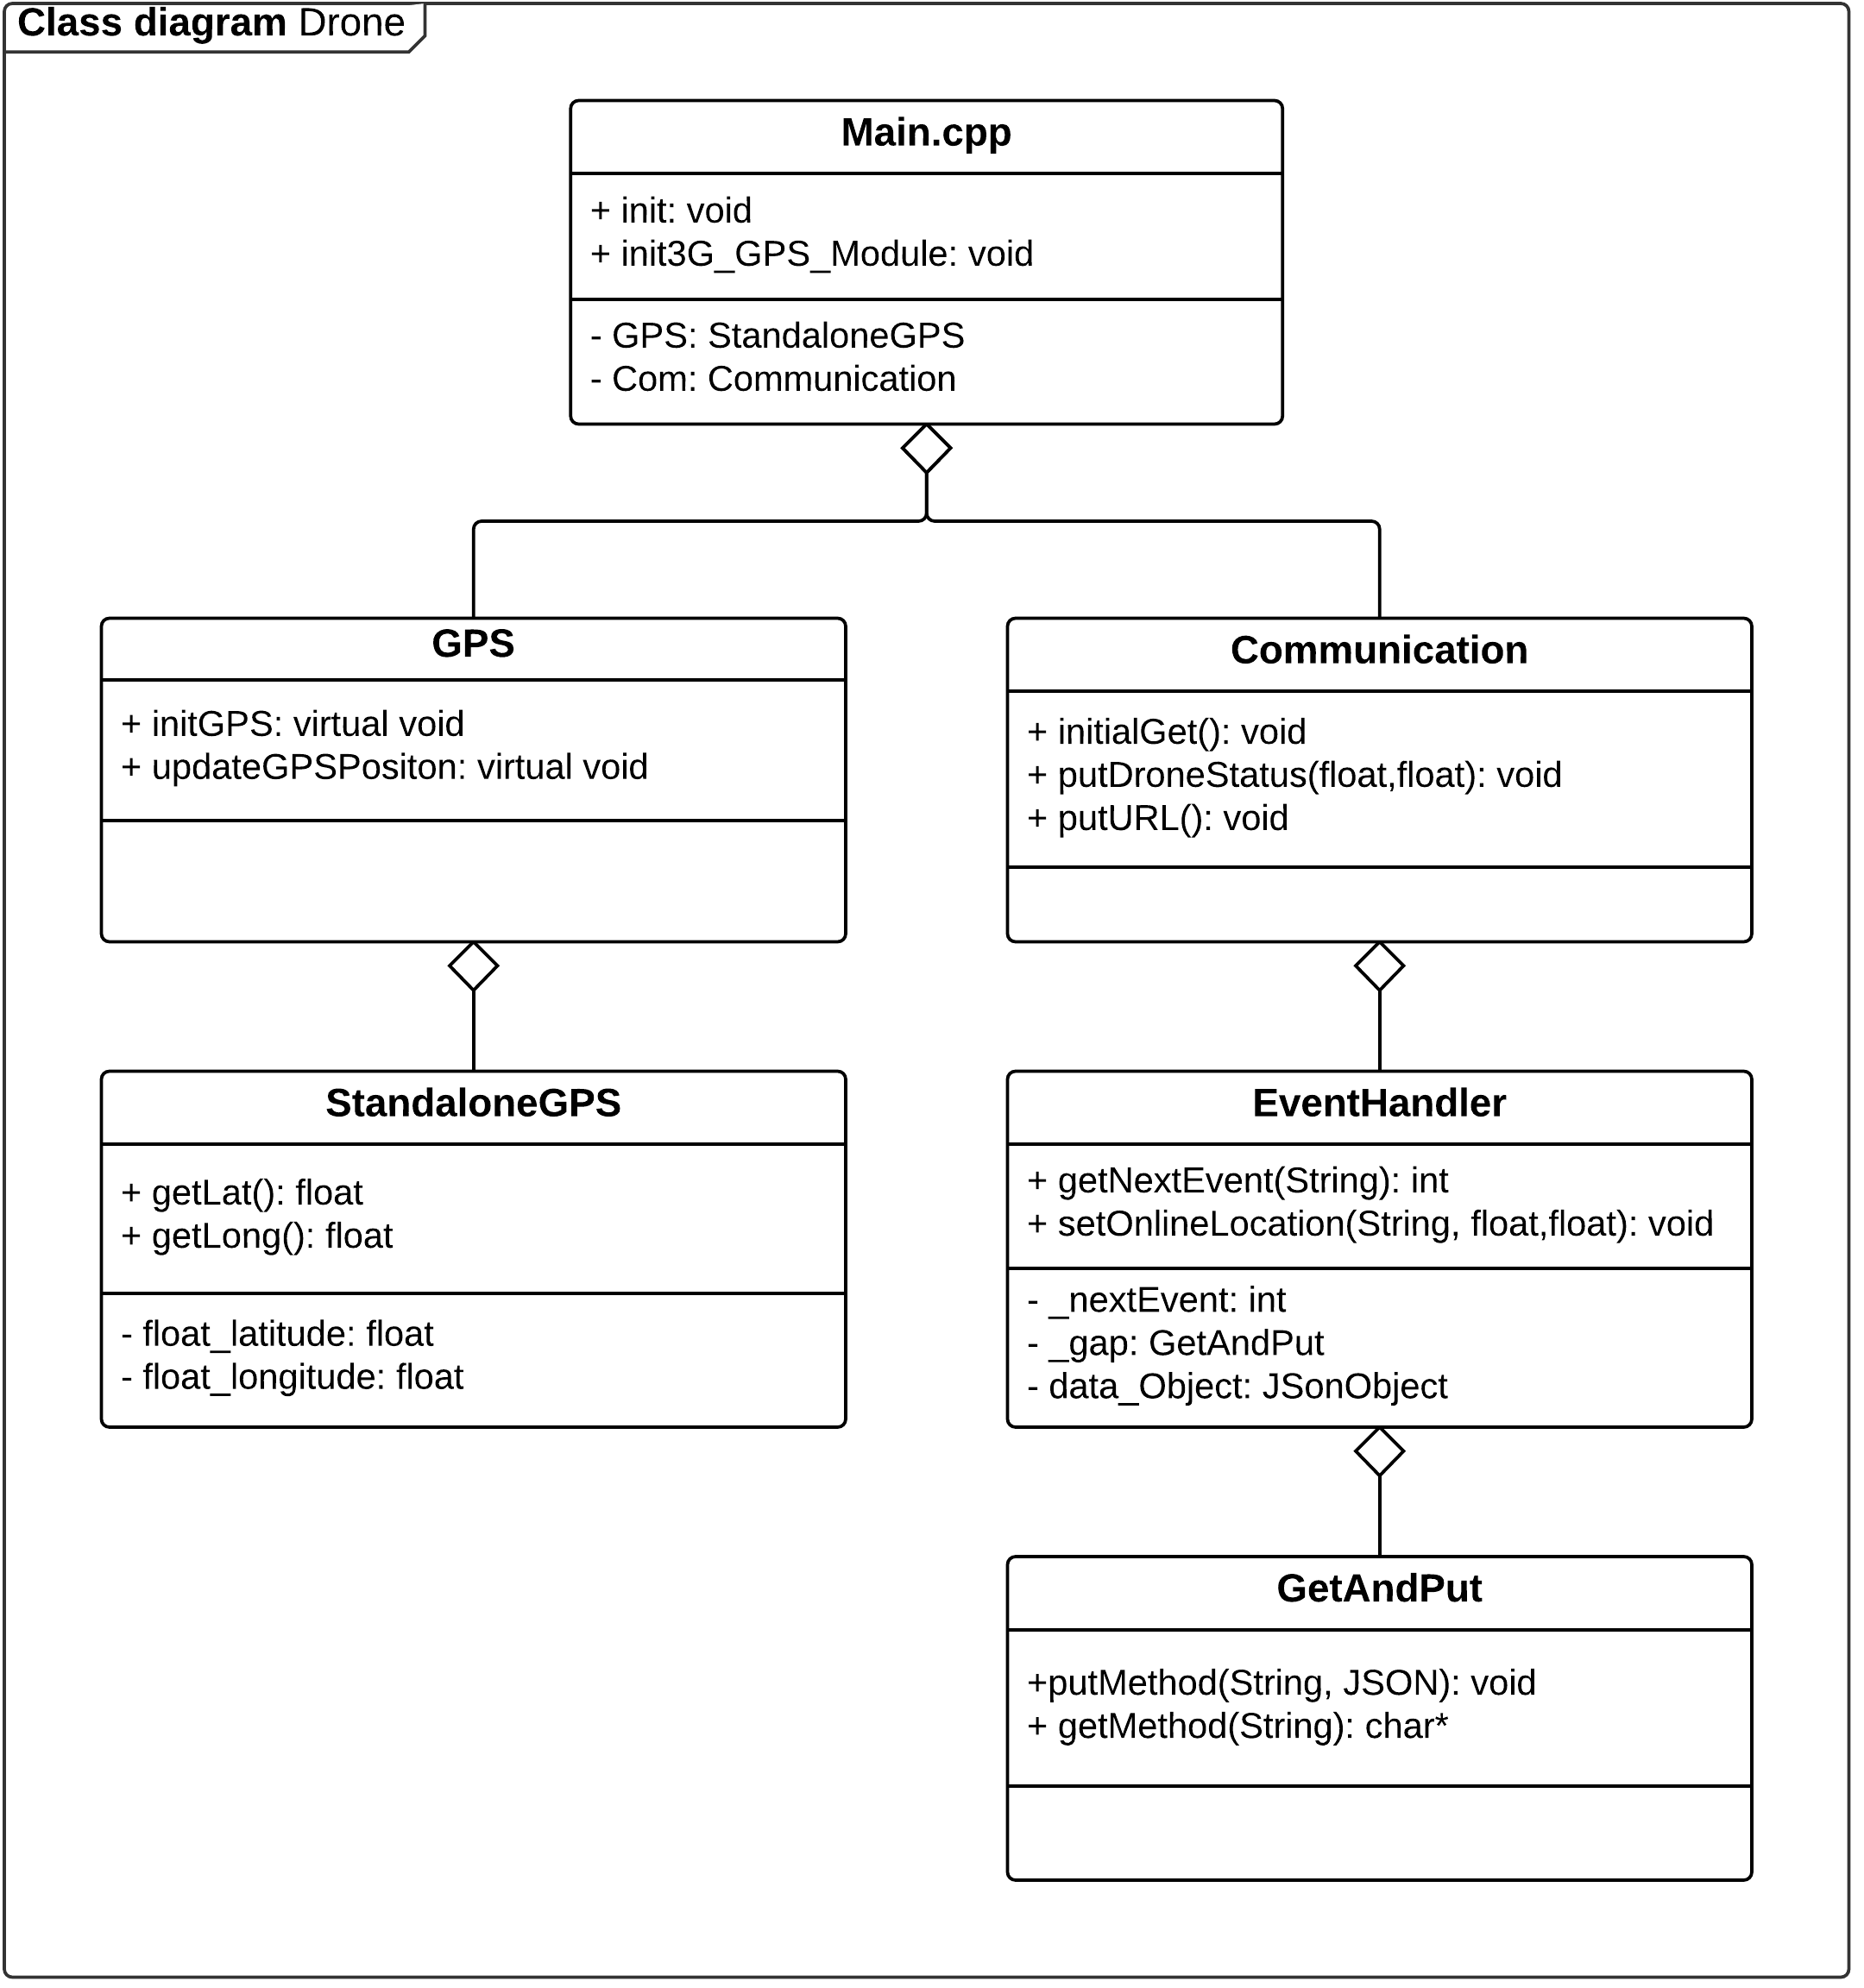
\includegraphics[width=1\textwidth]{Billeder/klasse_diagrammer/classdiagram_iteration1.png}
	\vspace{-0.5cm}
	\caption{Klassediagram \#iteration 1}
	\label{fig:classDiagram_iteration1}
\end{figure}
\vspace{-0.1cm}

\textbf{Main.cpp} \\
Main.cpp filen bruges til at sætte arduino board korrekt op, bla. sættes baudrate på de forskellige serielle forbindelser. Desuden bruges Main.cpp til at kalde og eksekverer forskellige klasse, objekter og funktioner.

\textbf{GPS} \\
GPS klassen er implementeret som en abstract klasse, idet den ikke selv har nogle metoder den skal bruge, men med virtuelle metoder der sikrer at de implementeres i de afledte klasser. 
Init og updateGPSPosition er valgt til at være virtuelle klasser, hvilket gør at de skal implementeres uanset hvilken GPS der bruges. Klassen er lavet fordi der i udgangspunkt var mulighed for at bruge 3 forskellige slags GPS modes med 3G/GPS shieldet. 

\textbf{StandaloneGPS}\\
Denne klasse er ansvarlig for al kommunikation med GPS'en når standalone mode er valgt. 

\newpage

Nedenfor ses figur \ref{fig:udvidet3G_it1} som er en udvidet klasse diagram over 3G modulet. Klasse diagrammet viser et udvidet klasse diagram, der viser hvilke metoder der indgår i iteration 1 for 3G modulet. 

\begin{figure}[H]
	\centering
	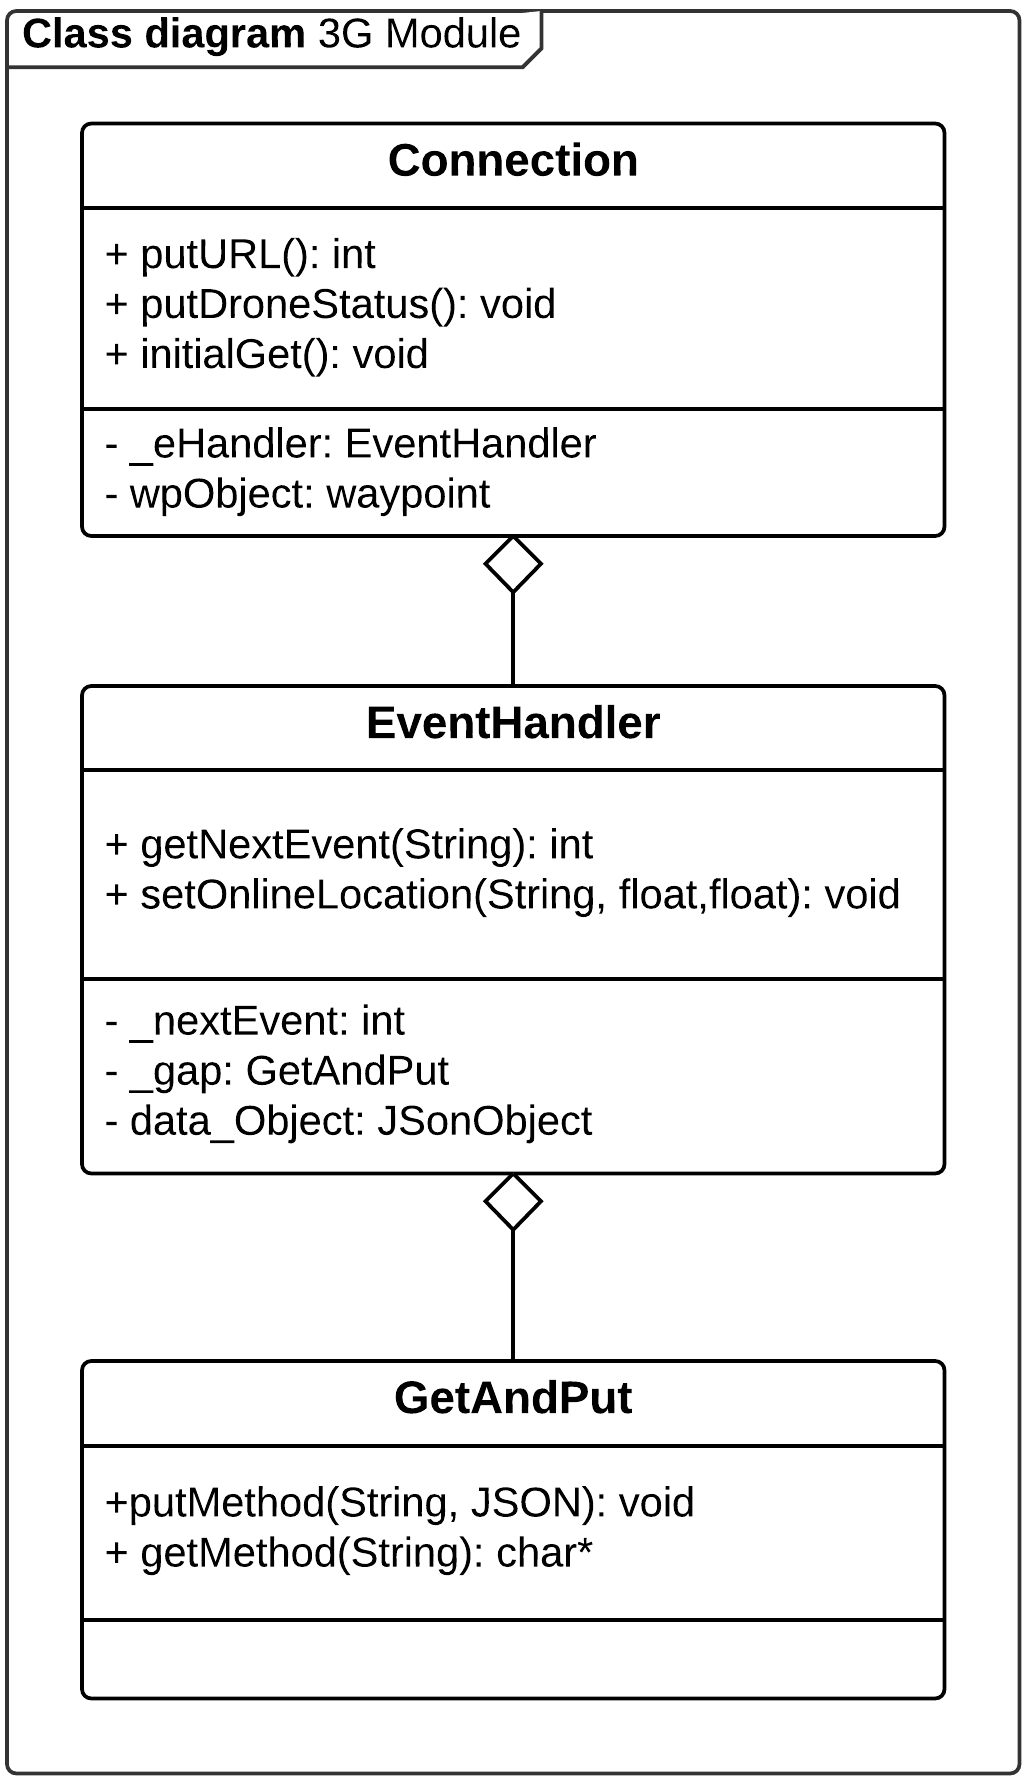
\includegraphics[width=0.50\textwidth]{Billeder/klasse_diagrammer/udvidet3G_iteration1.png}
	\vspace{0.5cm}
	\caption{Udvidet klasse diagram for 3G modulet - iteration 1}
	\label{fig:udvidet3G_it1}
\end{figure}

\textbf{GetAndPut} \\
GetAndPut klassen er den klasse der er tættest på hardwaren. Klassen indeholder de http metoder der bruges til kommunikation mellem dronen og serveren. 

\textbf{Communication} \\
Communication klassen er den øverste klasse og den håndterer sammen med andre klasser, alt der har med 3G at gøre.

\textbf{EventHandler} \\
EventHandleren er den klasse der håndterer Events. EventHandleren er bindeledet mellem communication- og GetAndPut klassen. EventHandleren sorterer eventID'et fra de data den modtager og returnerer værdien til communication klassen. 


\newpage

\subsubsection*{Klasse diagram - website}
\vspace{-0.2cm}
Figur \ref{fig:classDiagram_login} viser klassediagrammet tilhørende websitet for iteration 1.
\vspace{-0.2cm}
\begin{figure}[H]
	\centering
	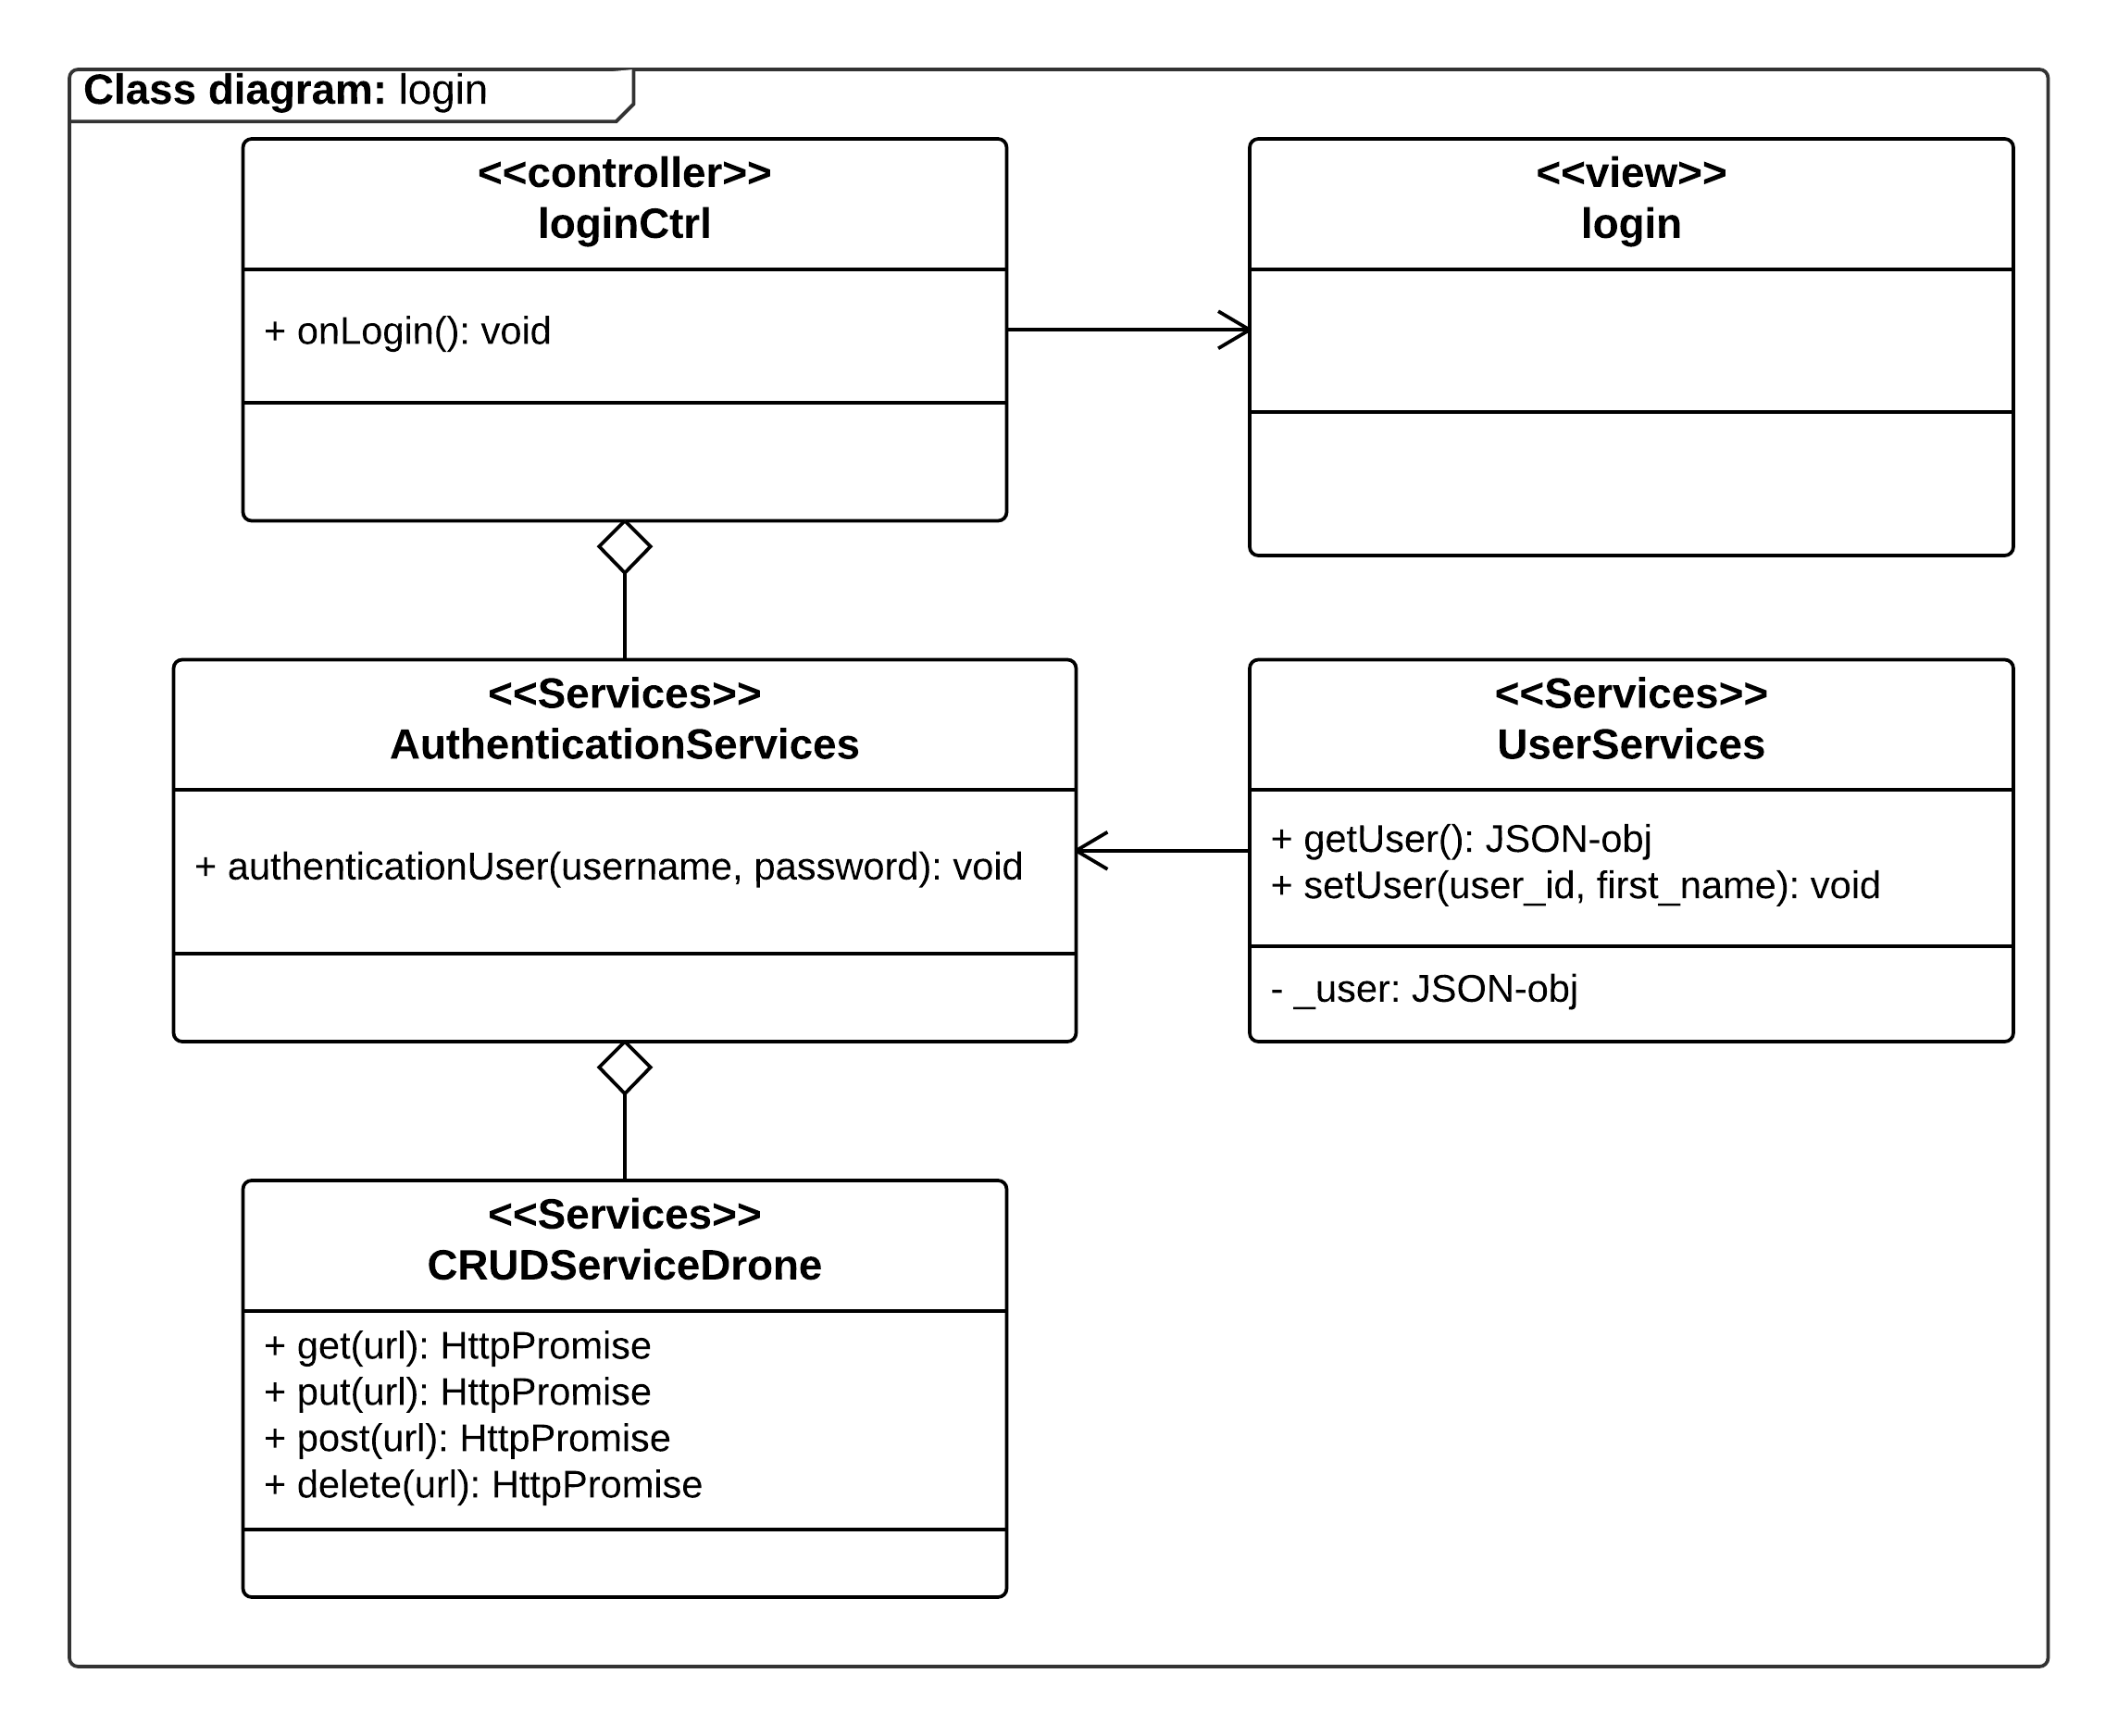
\includegraphics[width=1\textwidth]{Billeder/klasse_diagrammer/login_class_diagram.png}
	\vspace{-0.5cm}
	\caption{Klassediagram login}
	\label{fig:classDiagram_login}
\end{figure}

\vspace{-0.2cm}

\textbf{login} \\
Login view filen er det html script som useren ser på sin webclient. Filen er two-way databinded med loginCtrl klassen. Via denne binding kan der sendes og modtages data direkte.

\textbf{loginCtrl} \\
LoginCtrl er controller klassen som er forbundet med view klassen via two-way databinding. Klassen uddelegere også opgaver til dens services.

\textbf{AuthenticationServices} \\
AuthenticationServices er en service der afgør om user er authenticated eller ej. Hvis user er authenticated bliver han redirected til websitets home-page. Klassen gør brug af UserServices til at gemme information om den user der er logget ind i systemet.

\textbf{UserServices}\\
UserServices indeholder information om user der er logget ind i systemet.

\textbf{CRUDServiceDrone} \\
CRUDServiceDrone er den service der styre alt kontakt til databasen i systemet. Igennem denne service er det muligt at hente, opdater og poste data til databasen.



\newpage
\subsubsection*{Sekvens diagram - drone}
På sekvensdiagrammet på figur \ref{fig:Sekvens_diagram_iteration1}, vises hvilke klasser der indgår og bruges i første iteration. Af sekvensdiagrammet fremgår det, at sekvensen først startes når bruger tilslutter batteri og tænder dronen. Når der er tilkoblet forsyning initialiseres main controller samt 3G/GPS og nuværende GPS position  (longitude og latitude) opdateres. Dronens nuværende GPS position opdateres når dronen sender PUT requests til websitet. PUT requests bruges dels til at fortælle websitet at dronen er online og dels til at give websitet information om dronens nuværende position. 


%kommentar
\begin{figure}[H]
	\centering
	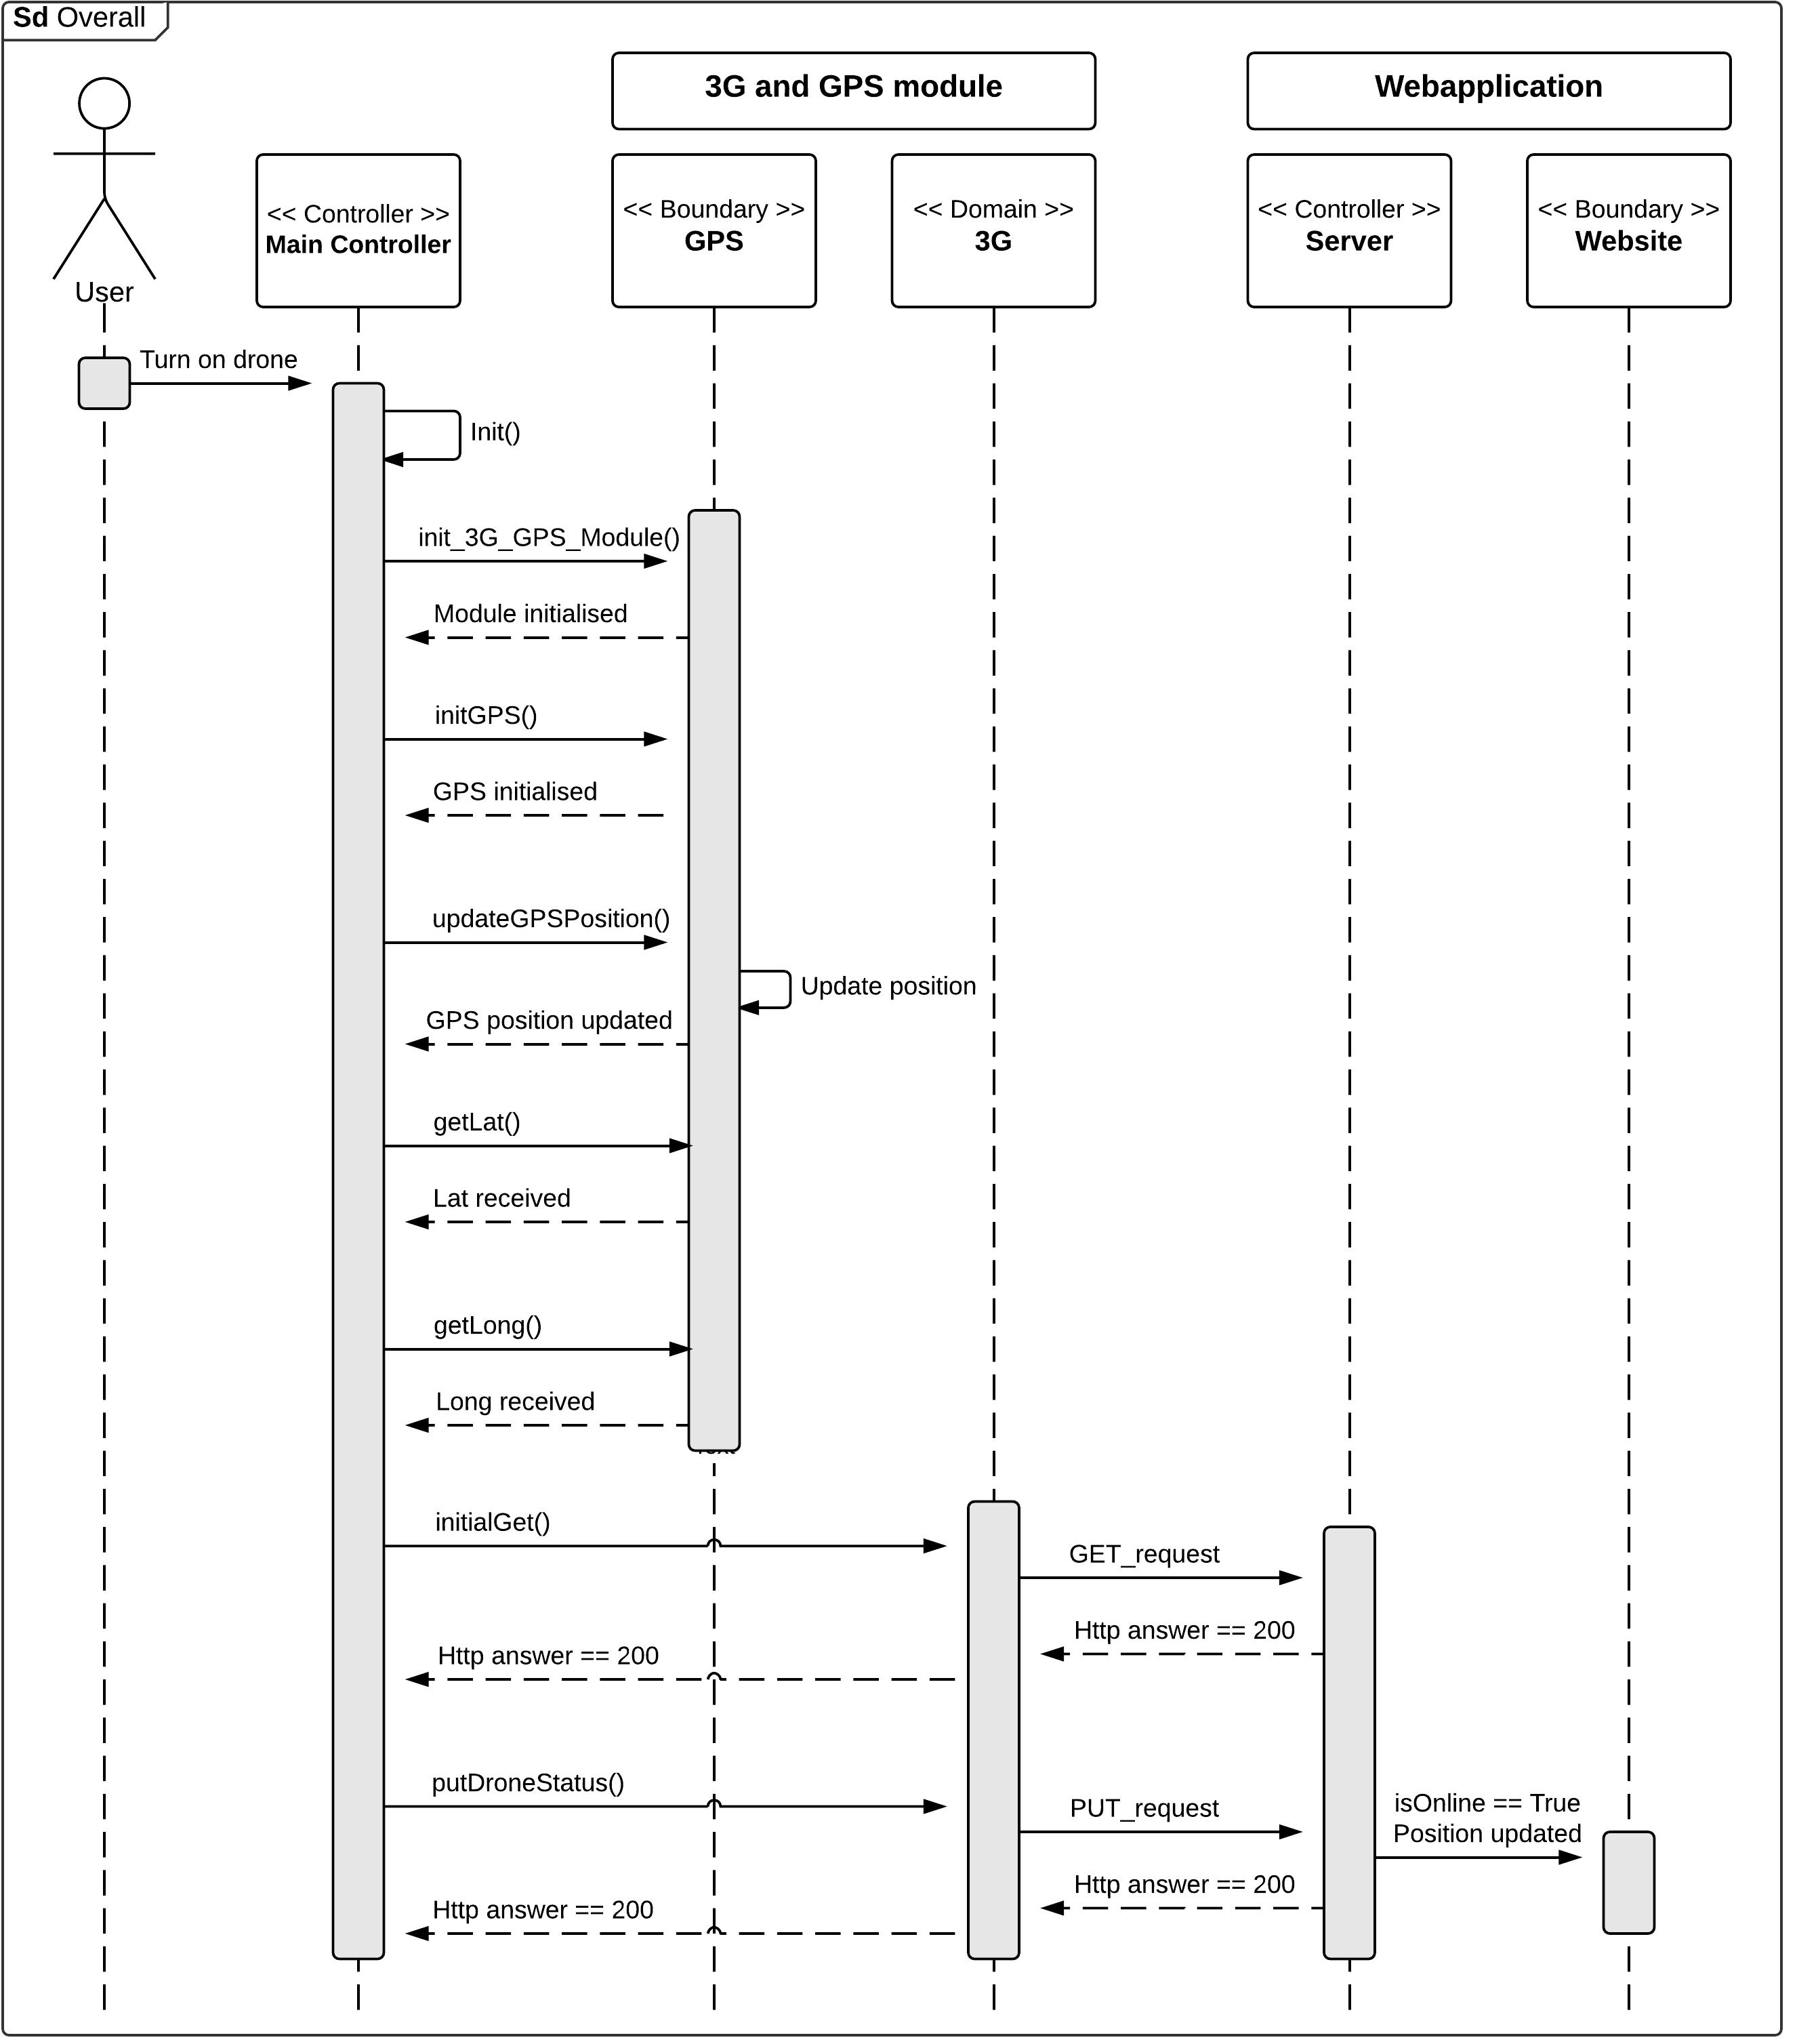
\includegraphics[width=0.93\textwidth]{Billeder/sekvens/sekvens_iteration1}
	\caption{Sekvens diagram \#iteration 1}
	\label{fig:Sekvens_diagram_iteration1}
\end{figure}
\newpage

På figur \ref{fig:Sekvens_diagram_initialget} og figur \ref{fig:Sekvens_diagram_putDroneStatus} bliver 3G modulet uddybet yderligere ifht. iteration 1.
\ref{fig:Sekvens_diagram_initialget} viser hvilke klasser der anvendes til at hente værdier fra serveren. De data der hendes ned med GET requesten, skal bruges sammen med PUT request i den anden klasse. For at kunne udføre et PUT funktion, skal de id'er der ønskes at blive sendt stemme overens med dem der ligger på serveren.

\begin{figure}[H]
	\centering
	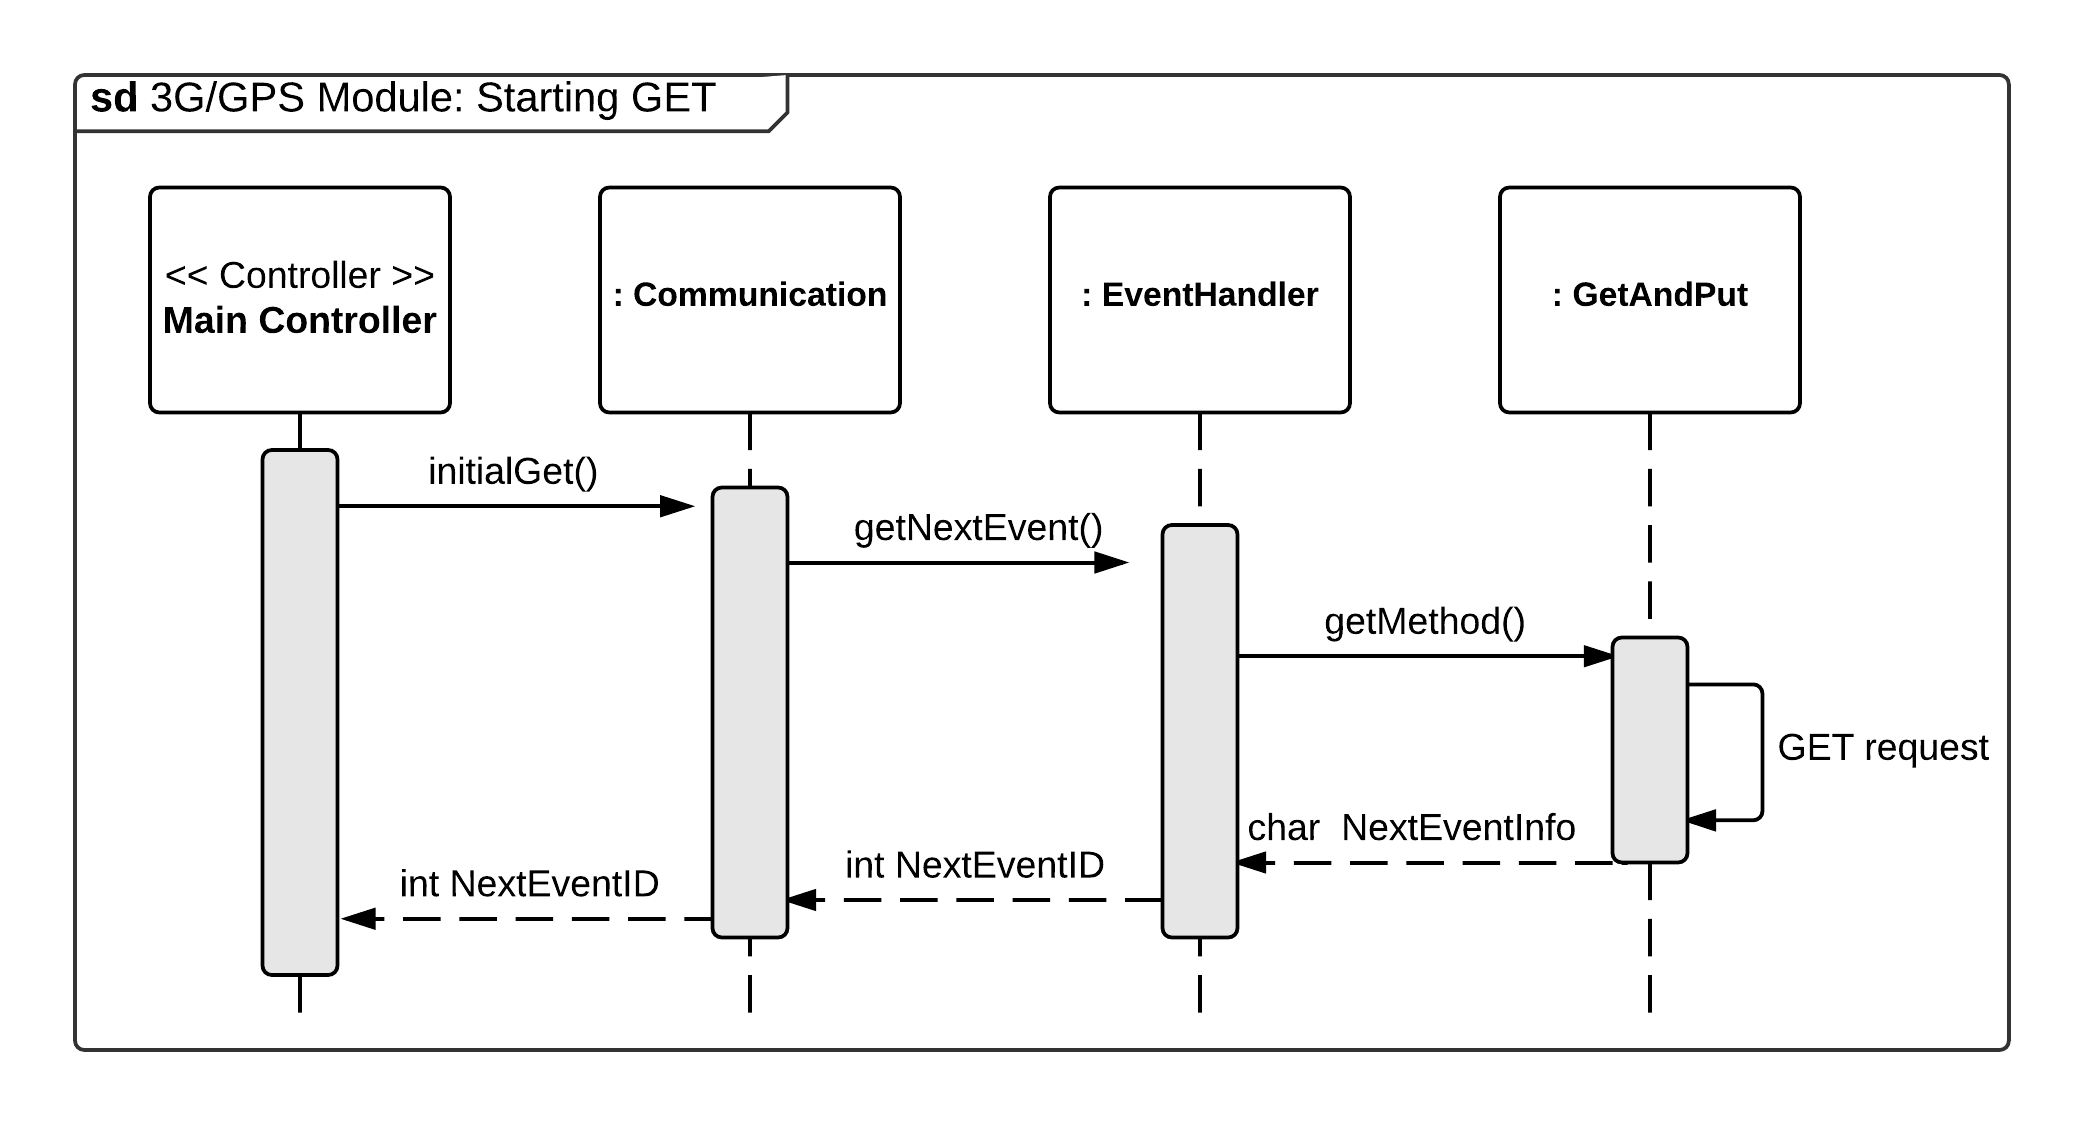
\includegraphics[width=0.93\textwidth]{Billeder/sekvens/sekvens_iteration1_initialget}
	\caption{Sekvens diagram \#iteration 1 - initialget}
	\label{fig:Sekvens_diagram_initialget}
\end{figure}

\begin{figure}[H]
	\centering
	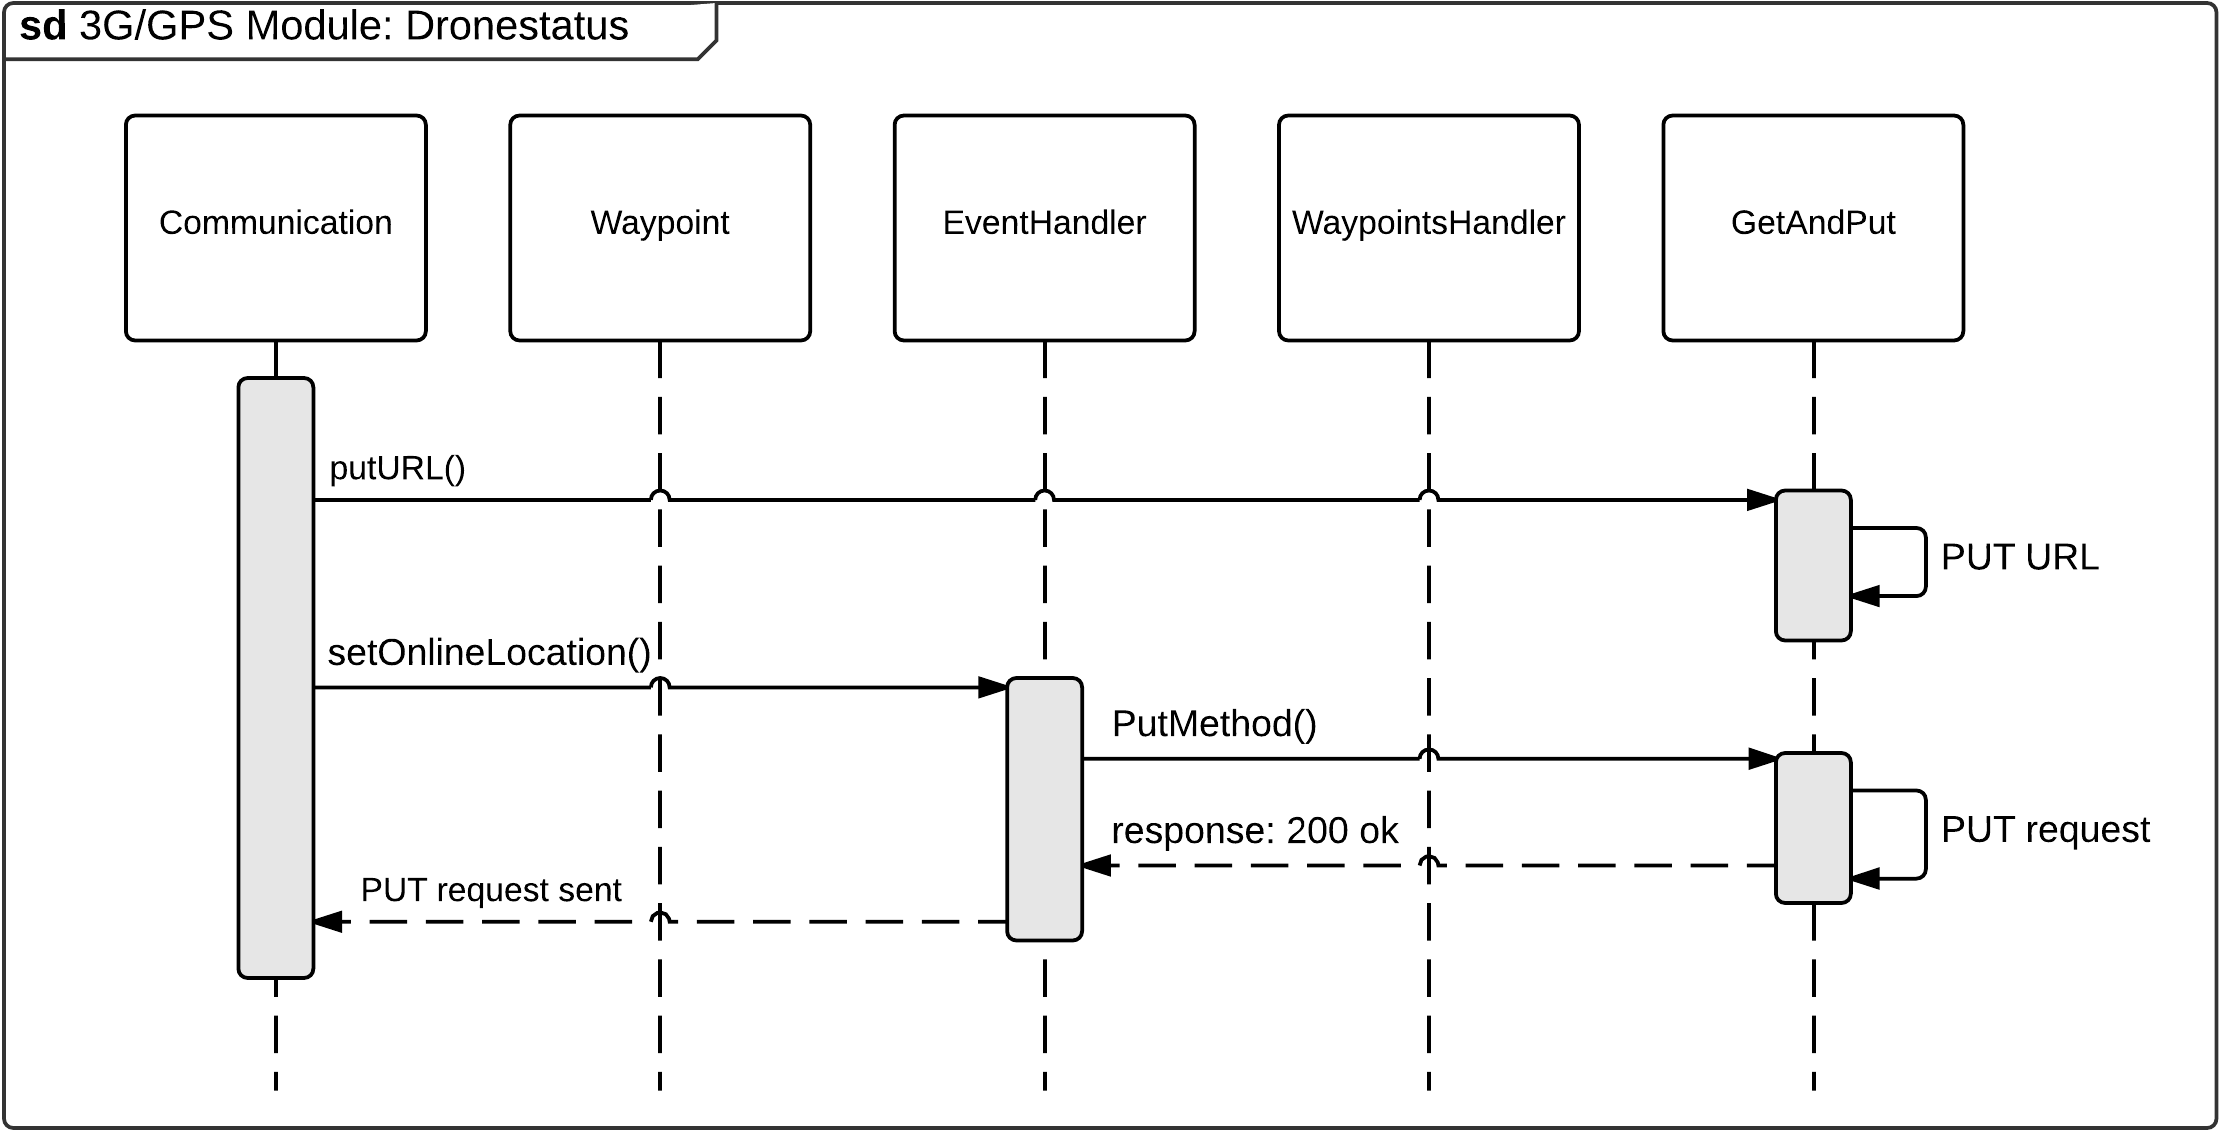
\includegraphics[width=0.93\textwidth]{Billeder/sekvens/sekvens_iteration1_putdronestatus}
	\caption{Sekvens diagram \#iteration 1 - putDroneStatus}
	\label{fig:Sekvens_diagram_putDroneStatus}
\end{figure}

\subsubsection*{Sekvens diagram - website}
På figur \ref{fig:Sekvens_diagram_login} ses sekvens diagrammet over login på websitet. På diagrammet vises det at useren først bliver ført til næste side ved succesfuld login. Diagrammet viser også kommunikationen med CRUDServiceDrone som kommunikerer med databasen. Diagrammet viser også hvordan AuthenticationServices setter den givet users data inden useren bliver ført vider i systemet.
\begin{figure}[H]
	\centering
	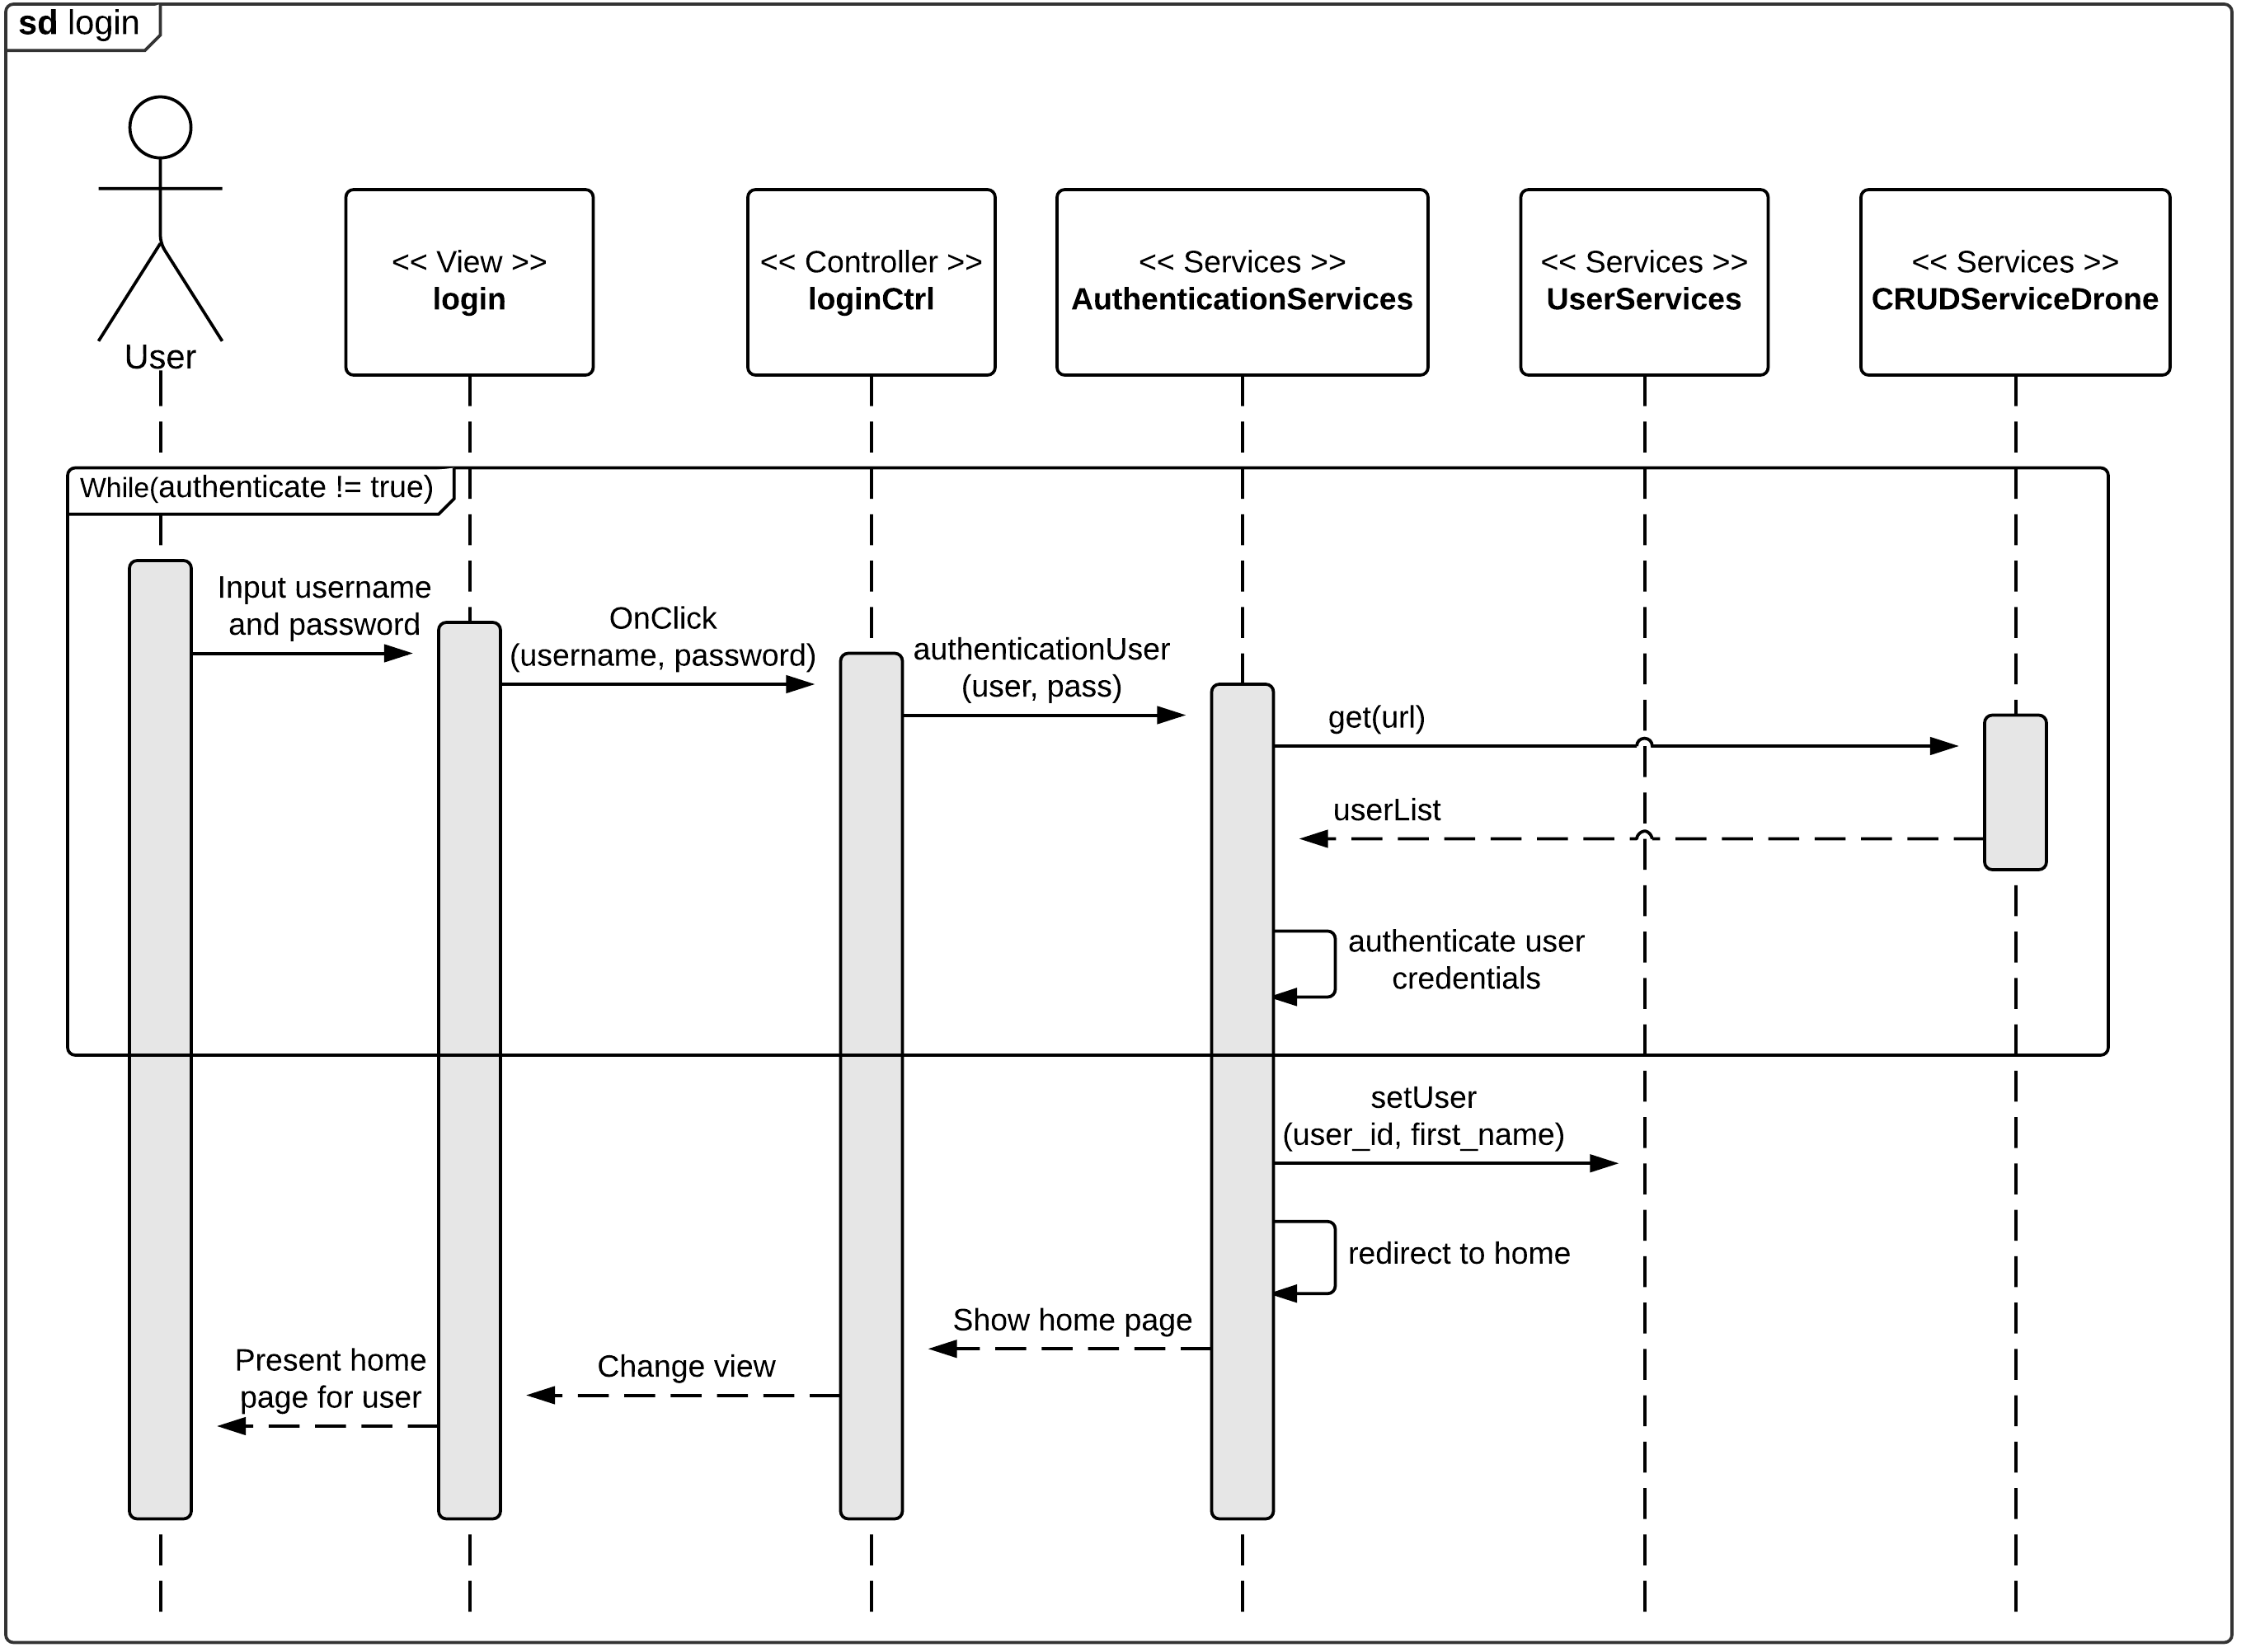
\includegraphics[width=0.93\textwidth]{Billeder/sekvens/login_sq_diagram.png}
	\caption{Sekvens diagram login}
	\label{fig:Sekvens_diagram_login}
\end{figure}
\newpage




\subsubsection*{State machine diagram}
\vspace{-0.1cm}
I state machine diagrammet på figur \ref{fig:Statemachine_iteration1}, vises de forskellige states der eksisterer i iteration 1 og hvordan flowet imellem dem ser ud. Der eksisterer givet vis kun 2 states i iteration 1, men state machinen er medtaget fordi den på nem og overskuelig vis illustrerer systemflowet.
%kommentar
\begin{figure}[H]
	\centering
	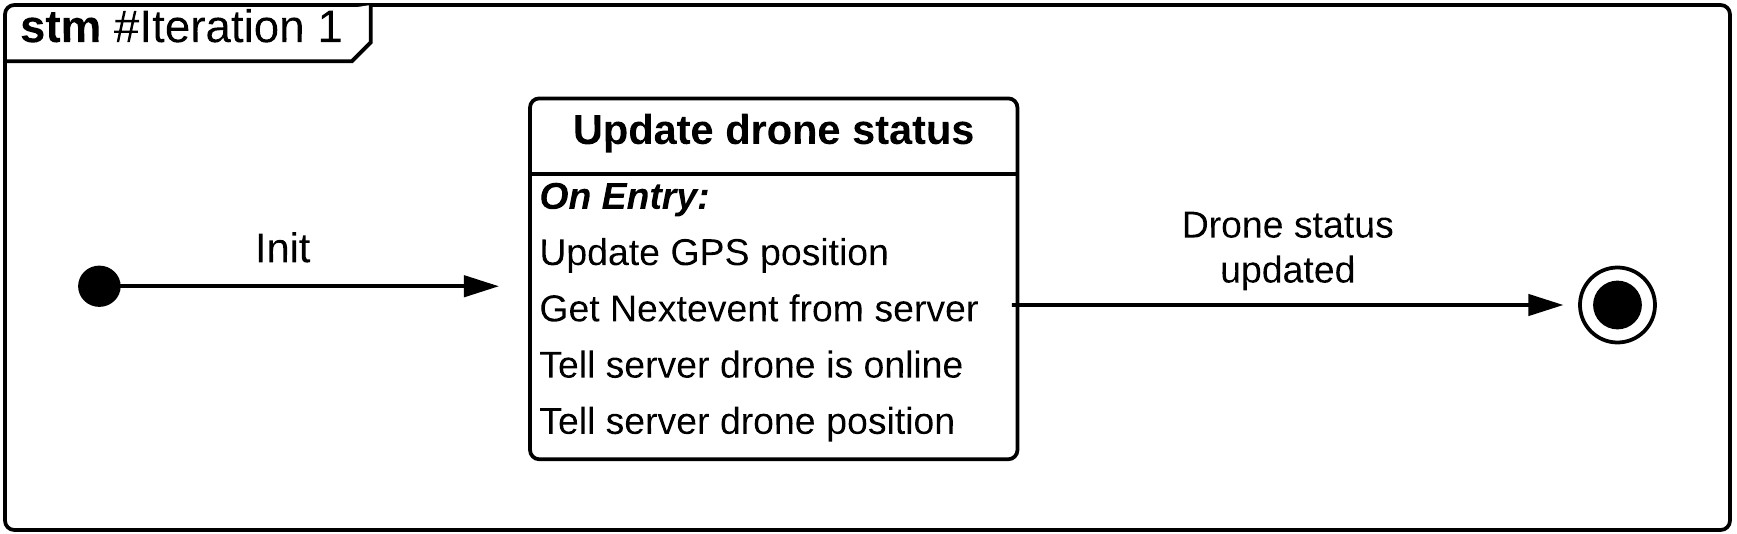
\includegraphics[width=1\textwidth]{Billeder/statemachine/State_iteration1.png}
	\vspace{-0.5cm}
	\caption{Statemachine \#iteration 1}
	\label{fig:Statemachine_iteration1}
\end{figure}